\section{x86 Address Translation Basics}
The address a software uses to access information and
instructions is called a virtual address. Segment and offset
fields make up the virtual address. The segment
information is utilised to calculate the segment's starting
address and protection details. Although operating
systems typically employ flat segmentation, in which
every segment is mapped to the whole physical address
space, segment translation cannot be turned off. The
virtual address essentially becomes the linear address
under flat segmentation. \newline \newline
Linear and virtual addresses will be used interchangeably
in this paper. If paging is enabled, processor paging
hardware converts the linear address to a physical
address. The operating system generates and maintains a
collection of page tables in order to use paging as shown
in Figure 3. These page tables and different bit fields in
the linear address are used to execute address translation
by the page table walker, sometimes known as just the
page walker, which is implemented in processor
hardware. The high-level algorithm that the page walker
uses to translate addresses is depicted in Figure \ref{fig:virtual-to-physical-address-translation-algorithm}.\newline \newline
During the page walk, the page walker encounters
physical addresses in CR3 register and in page table
entries which point to the next level of the walk. When
the data or leaf page is reached, the page walk comes to
an end. Because the page walker must repeatedly visit the
memory hierarchy, address translation is a relatively
memory intensive operation. AMD processors
automatically retain recent translations in an internal
translation look aside buffer (TLB) to minimise this
overhead. The processor initially examines the TLB at
each memory reference to see if the necessary translation
is already cached. If it is, the processor uses that
translation, if not, page tables are traversed, the
translation is saved in the TLB, and the instruction is
carried out. To maintain consistency between the TLB
and page tables in memory, operating systems must work
with the CPU.
\begin{figure}[ht]
    \centering
    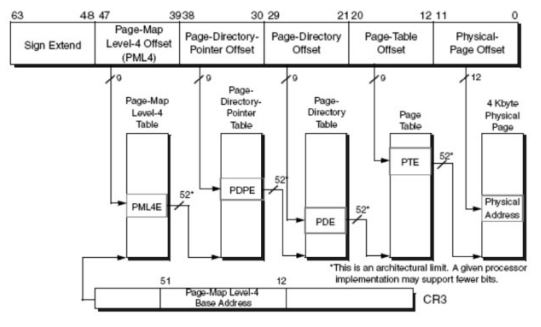
\includegraphics[width=\linewidth]{./images/4kb-page-tables-in-long-mode.png}
    \caption{4kb page tables in long mode}
    \label{fig:4kb_page_tables_in_long_mode}
\end{figure}
\newline
For example, the operating system must ask the processor
to invalidate the TLB record linked to the address
translation in order to remove it. The operating system
must guarantee that TLB entries on all processors stay
consistent on SMP systems, where an operating system
may share page tables amongst processes working on
multiple processors. Operating system software should
invalidate the associated TLB entry on each processor
when a shared translation is removed. During a context
switch, the operating system modifies the base pointer
(CR3) of the page table. The processor automatically
invalidates TLB entries linked to the previous context
when a CR3 modification creates a new set of
translations. During memory accesses, the processor
updates the page tables with accessed and dirty bits.
When the processor reads or writes to memory using that
translation, the "accessed" bit is set at every level of the
page table. When the CPU writes to the memory page that
the PTE maps, the PTE's "dirty" bit is set.
\begin{figure}[ht]
    \centering
    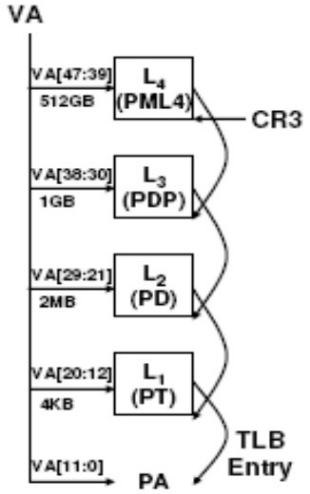
\includegraphics[width=\linewidth, height=0.3\textheight]{./images/virtual-to-physical-address-translation-algorithm.png}
    \caption{4kb page tables in long mode}
    \label{fig:virtual-to-physical-address-translation-algorithm}
\end{figure}